\chapter{Implementation Details}
Though developments in hardware enables us to exploit parallelism, but there is still a need to know about the implementation of the algorithms. Having the
vision for the implementation we can decrease overhead and improve performance. In the following sections some instances will be discussed where an
understanding of the implementation details [10] can be exploited to achieve better efficiency.

\section{Parallel Decomposition and Data Dependency Graphs}
Parallel computations can be described with the help of the control flow graphs [10]. Such a graph consists of nodes that represent processes and directed
edges that represent execution dependencies. These graphs can represent both fine-grain and coarse-grain parallelism, but these are best suited for the coarse
grain parallelism. In this case it is convenient to have the nodes represent serial subroutines or procedures that may execute in parallel. Leaves of such
graphs represent processes that may execute immediately and in parallel. The graph asserts that there are no data dependencies between leaf processes. That is,
there is no contention for write access to a common location between two leaf processes. The control flow representation of parallel computation differs from a
data flow representation in the sense that the edges of the control flow graph do not represent data items. Instead, these edges represent the assertion that
data
dependencies do not exist once there are no incoming edges. The programmer must take the responsibility for ensuring that the dependencies represented by the
graph are valid. For an example, the term execution dependencies means that one process is dependent upon the completion of, or output from, another process
and is unable to begin execution until this condition is satisfied. Additional processes may be dependent on this process. \par
\hspace{1in} A special case of the execution dependency is deadlock [2,10]. This phenomenon, encountered only in MIMD machines, is caused by a circular
dependency chain so that all activity ceases, with all processors either idle or in a wait state. This is the most difficult bug to detect or fix. In
particular, acyclic control flow graphs don't admit deadlocks. Thus, describing a parallel decomposition in terms of such a graph avoids this problem from the
outset. One example is shown in figure 3.1. This abstract representation of the parallel decomposition graph can easily be reformed into a parallel program.
A correct understanding of the data dependencies among communicating parallel processes is, of course, essential to obtain a correct parallel program.
Once these dependencies have been understood, a control flow graph can be constructed that will ensure that the data dependencies are satisfied. A control flow
graph may go further by introducing execution dependencies to force a particular order of computation if that is deemed necessary for the purpose of load
balancing or performance. 

\begin{figure}[ht]
{\centering \resizebox*{4in}{3in}{\includegraphics{lgrain.ps}} \par}
\caption{Large-Grain control flow graph}
\end{figure}

\section{Synchronization}
Synchronization [1,2,10] is required when two or more concurrently executing process must communicate, to signal their completion to each other, or simply to
provide information to the other of its current progress. The crudest and most common form of synchronization is that of the barrier often used in the join of
a fork-and-join. Here a task records its completion and halts. Only when all of the processes have reported to the barrier, the task halted at the barrier
can continue further.\par
\hspace{1in} Most shared memory processors use lock function [1] for the synchronization. A lock function tests the value of the lock variable. If the value is
on, the process is blocked until the lock variable is off. When the lock variable is found to be off, it is read and set to on in an autonomous operation.
Thus, exactly one process may acquire a lock variable and set it to on. A companion to a lock function is an unlock function, which serves to set the lock
variable to off. When a task wishes to have exclusive use of a section of the code (or exclusive use of data accessed), it tries to set the lock through a
subroutine call. In this situation a programmer has a section of program that is to be executed by at most one process at a time, called a critical section. If
the lock has already been set by another task, it is unable to set the lock and continue into the critical section, until the task, that sets a particular lock
unsets or unlocks it. An example of the locks, unlocks and critical section is given below:

\begin{verbatim}

            CALL LOCK( <lock variable> )
                   execute critical section
            CALL UNLOCK( <lock variable> )

\end{verbatim}
A more flexible and powerful form of synchronization can be achieved through the use of {\it events} [1]. Events can be posted, awaited, checked for, and
unposted. Any processor can unpost an event, and after checking its existence, the programmer is free to continue if appropriate. This form of synchronization
is becoming increasingly common.

\section{Load balancing}
Load balancing [1,10] involves allocating tasks to processors so as to ensure the most efficient use of resources. With the advent of parallel processing, the
ability to make iterations of loops run in parallel, refered to as microtasking, has become increasingly important. It can be very efficient to split off even
small tasks: the determining factor is whether wall clock time has been reduced without having to pay significantly more for the increase in CPU time
(resulting from parallel overhead).\par
\hspace{1in} When a job is multiprocessed, a common measure of efficiency is the ratio of the elapsed time on one processor to that on $p$ processors divided
by the $p$. This ratio reflects both time lost in communication or synchronization and idle time on any of the $p$ processors. It is the idle time that load
balancing strategies seek to minimize. \par 
\hspace{1in}For an example, to illustrate the effect of load balancing, let us assume that there are four processors and seven independent tasks, which
simultaneously make one work. Let one of the tasks requires 2 units of time and rest takes 1 unit of time each. Then, an optimized distribution of the tasks
will be such that three processors get six tasks of 1 unit of time, each having two tasks and fourth one has the task of 2 unit time. In this way the work will
be completed in the 2 unit of time. Any other partition of tasks will take more time than the previous partition. \par
\hspace{1in} Suppose we take a system, that is multiprogrammed, if one or more processors are idle, that should not be of great concern since the idle time can
be taken by another job. This point is of particular importance when the parallelism, measured in the number of simultaneously executable tasks, varies during
the course of a job. Thus it might be efficient at one time to use all the processors of a system while at another time to use only one or two processors.
Finally, it is observed that on a highly parallel machine, many tasks are required to saturate the machine, so that the problem size has to be large enough to
generate enough parallelism.
